% PLaMo Paper Translator user manual, typeset as an academic paper.
% Dedicated to the public domain under CC0 1.0. See README.md in this folder.
\documentclass[10pt,twocolumn]{article}
\usepackage[T1]{fontenc}
\usepackage{mathptmx}
\usepackage[margin=0.75in,columnsep=0.28in]{geometry}
\usepackage{amsmath,amssymb}
\usepackage{graphicx}
\usepackage{booktabs,multirow}
\usepackage{caption,subcaption}
\usepackage{algorithm,algpseudocode}
\usepackage[hidelinks]{hyperref}
\captionsetup{font=small,labelfont=bf}
\graphicspath{{figures/}}

\title{\textbf{PLaMo Paper Translator: Local, Sentence-Aligned\\Bilingual Reading of Academic PDFs}\\[4pt]
\large User Manual, Version 1.1}
\author{The PLaMo Paper Translator Project}
\date{November 2026}

\begin{document}
\maketitle

\begin{abstract}
PLaMo Paper Translator is a desktop application that turns an academic PDF into a sentence-aligned bilingual document and keeps everything on the reader's own computer. The application extracts text, figures and numbered equations from the PDF, translates each sentence with PLaMo 3 Translate running locally through llama.cpp, and presents the result in a three-pane reader with a table of contents, cross-reference links, bookmarks, notes and pinned clips. This manual is written in the form of a research paper so that it can double as a realistic test document: it contains numbered sections, figures, tables, display equations, an algorithm and a reference list. We describe installation (Section~\ref{sec:install}), the document pipeline (Section~\ref{sec:pipeline}), translation (Section~\ref{sec:translation}), the reading interface (Section~\ref{sec:reader}), quality checks (Section~\ref{sec:quality}) and the paper library (Section~\ref{sec:library}).
\end{abstract}

\noindent\textbf{Keywords:} machine translation, PDF processing, local inference, reading interface, PLaMo

\section{Introduction}
\label{sec:intro}
Reading papers in a second language is slow, and pasting text into an online translator breaks figures, equations and the structure of the document. Many papers are also confidential before publication, which rules out cloud services. PLaMo Paper Translator addresses both problems. All processing happens on the local machine, and the original structure of the paper is preserved: headings become a table of contents, figures and equations stay next to the text that refers to them, and every sentence is shown beside its translation.

Figure~\ref{fig:reader} shows the reader. The original text appears on the left, the translation in the middle and the reader's notes on the right. Each row is one segment, labelled with its paragraph and sentence number.

\begin{figure*}[t]
  \centering
  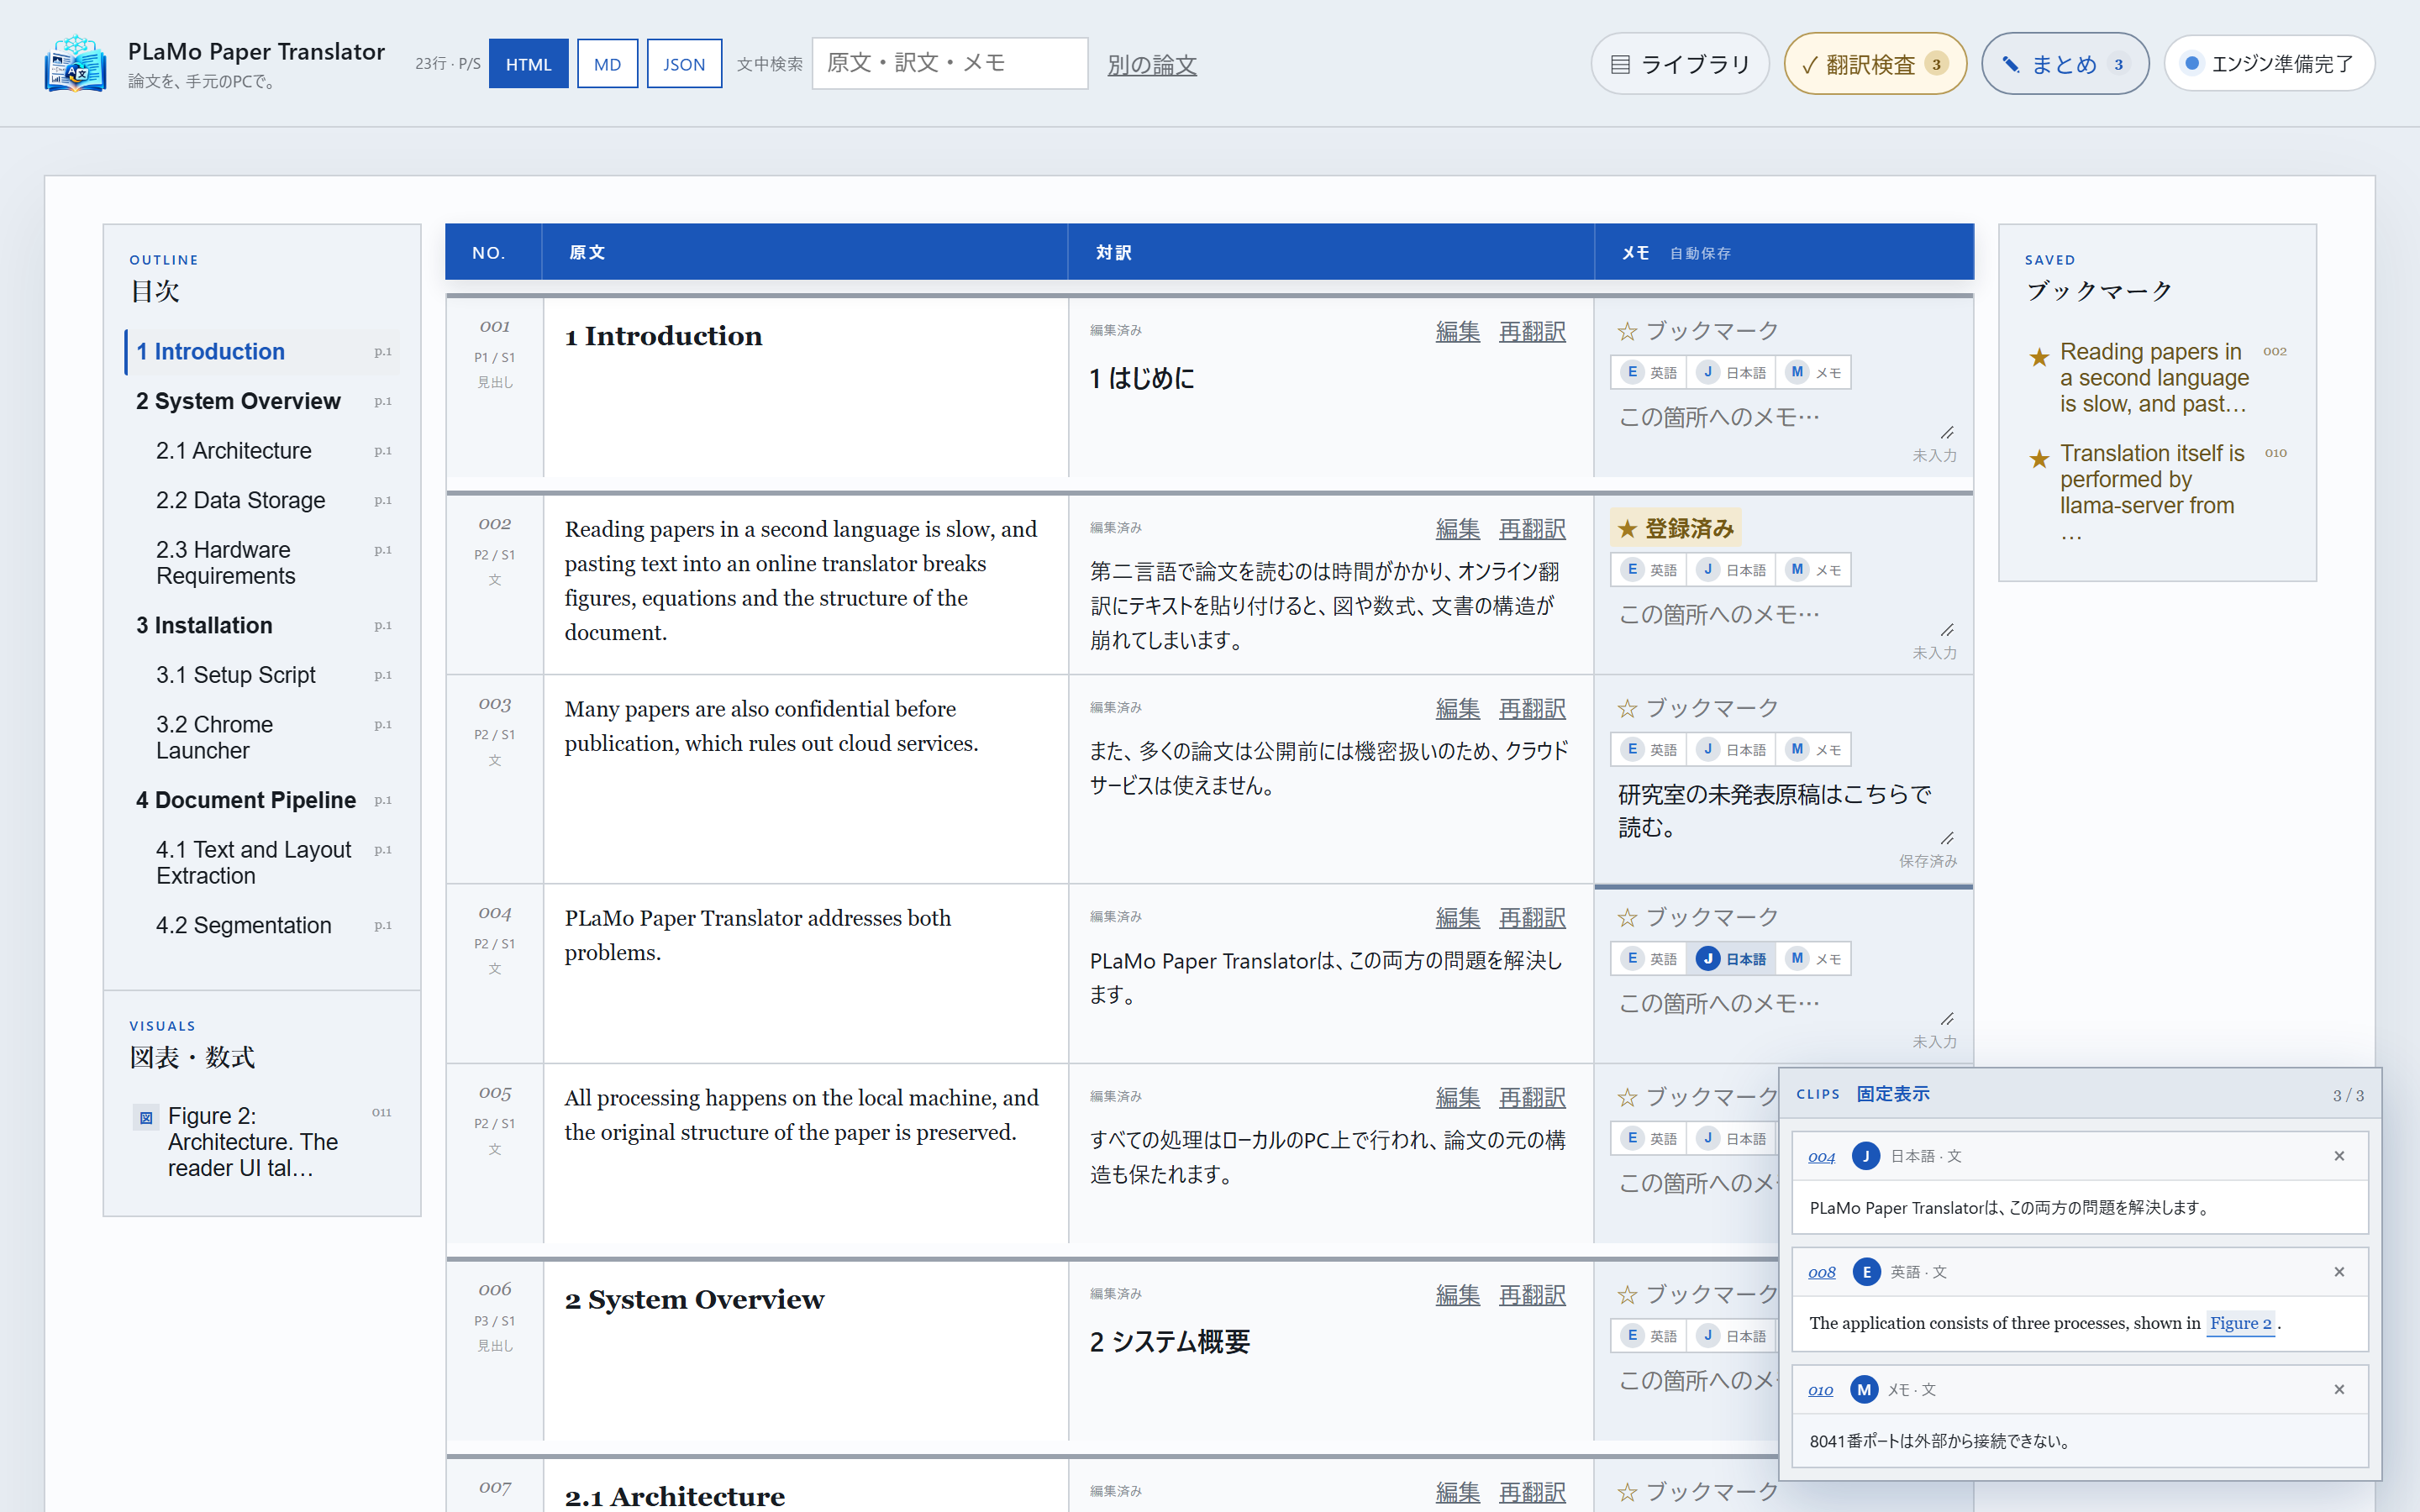
\includegraphics[width=\textwidth]{fig-reader.png}
  \caption{The reading interface. The outline (left) is generated from the section structure of the paper. Each row pairs one source sentence with its translation and a note field; the bookmark list is shown on the right.}
  \label{fig:reader}
\end{figure*}

The main contributions of the application are as follows.
\begin{itemize}
  \item A fully local pipeline that needs no network connection after the first setup.
  \item Structure-aware extraction that keeps headings, captions, numbered equations and reference entries intact.
  \item Context-aware translation that sends neighbouring sentences from the same paragraph to the model.
  \item A research-oriented reader with cross-reference jumps, notes, bookmarks, clips, a quality check and a searchable library.
\end{itemize}

\section{System Overview}
\label{sec:overview}

\subsection{Architecture}
The application consists of three processes, shown in Figure~\ref{fig:architecture}. A browser displays the reader UI. A small Python HTTP server, \texttt{app.py}, listens on \texttt{127.0.0.1:7865}; it extracts documents, runs translation jobs and stores results. Translation itself is performed by \texttt{llama-server} from llama.cpp~\cite{llamacpp}, which serves the PLaMo 3 Translate model~\cite{plamo3} on \texttt{127.0.0.1:8041}. Both servers bind to the loopback interface only, so no other computer can reach them.

\begin{figure*}[t]
  \centering
  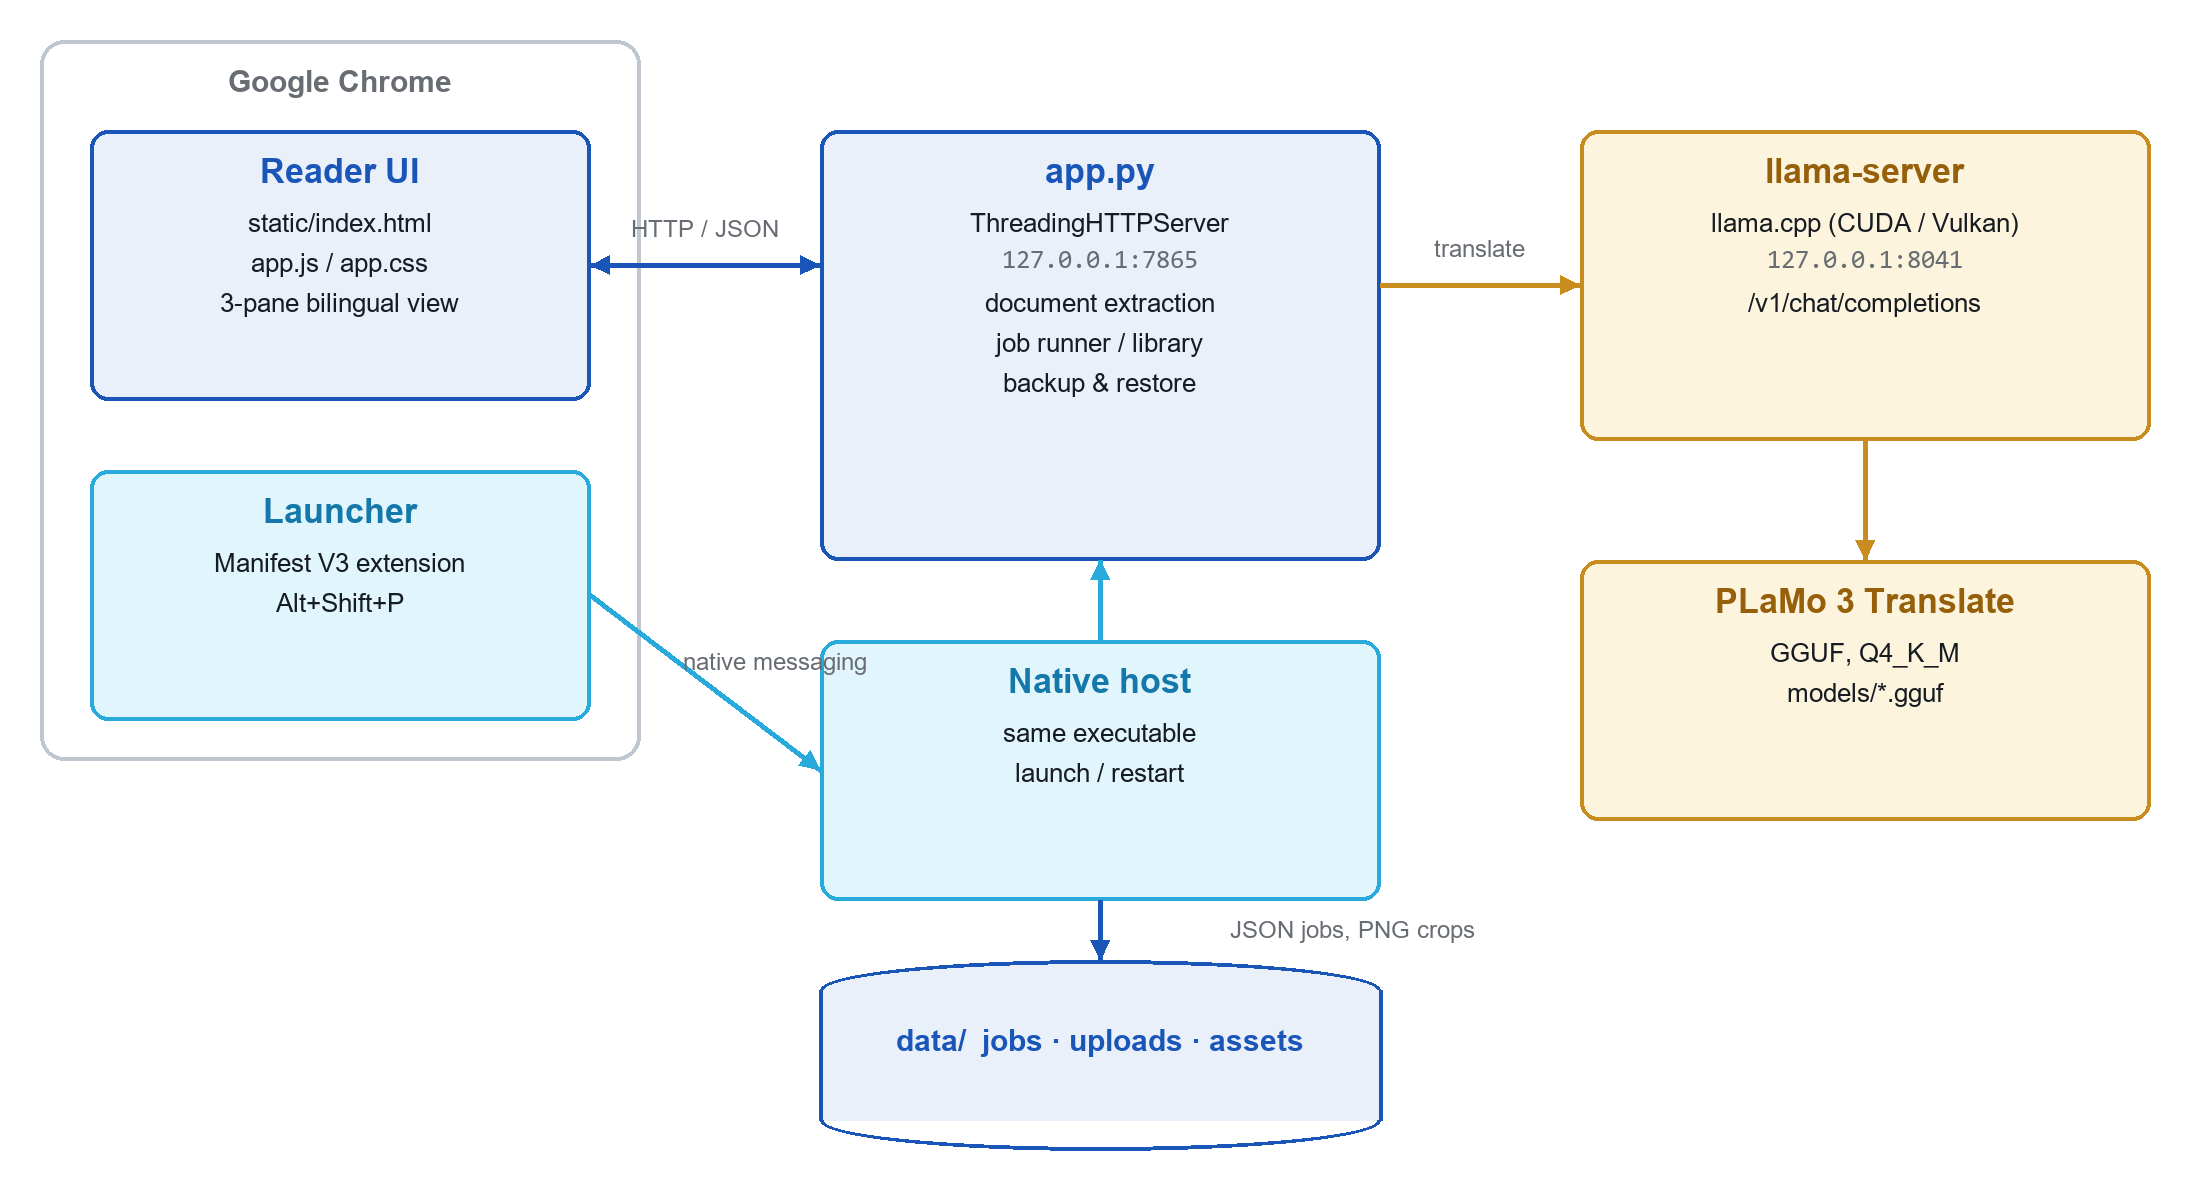
\includegraphics[width=0.92\textwidth]{fig-architecture.png}
  \caption{Architecture. The reader UI talks to \texttt{app.py} over HTTP; \texttt{app.py} calls llama-server through its OpenAI-compatible endpoint. The optional Chrome launcher starts or restarts the application through native messaging.}
  \label{fig:architecture}
\end{figure*}

\subsection{Data Storage}
All user data is kept in plain files under a single folder, summarised in Table~\ref{tab:storage}. Deleting the folder removes every trace of a paper.

\begin{table}[t]
  \centering
  \caption{Folders used by the application.}
  \label{tab:storage}
  \begin{tabular}{@{}ll@{}}
    \toprule
    Folder & Contents \\
    \midrule
    \texttt{data/uploads} & original PDF, TXT or Markdown \\
    \texttt{data/jobs} & one JSON file per translation \\
    \texttt{data/assets} & figure and equation crops (PNG) \\
    \texttt{models} & GGUF model and chat template \\
    \texttt{runtime} & llama.cpp binaries \\
    \bottomrule
  \end{tabular}
\end{table}

\subsection{Hardware Requirements}
The reference machine has an NVIDIA RTX 2000 Ada laptop GPU with 16\,GB of video memory. Table~\ref{tab:models} and Figure~\ref{fig:models} compare the available quantised models. The 8B model is the default; the 31B model does not fit in 16\,GB.

\begin{table}[t]
  \centering
  \caption{PLaMo 3 Translate models in Q4\_K\_M quantisation.}
  \label{tab:models}
  \begin{tabular}{@{}lrrl@{}}
    \toprule
    Model & Size (GB) & Bytes & Fits 16\,GB \\
    \midrule
    2B & 1.81 & 1{,}807{,}203{,}040 & yes \\
    8B & 5.28 & 5{,}280{,}445{,}728 & yes (default) \\
    31B & 19.53 & -- & no \\
    \bottomrule
  \end{tabular}
\end{table}

\begin{figure}[t]
  \centering
  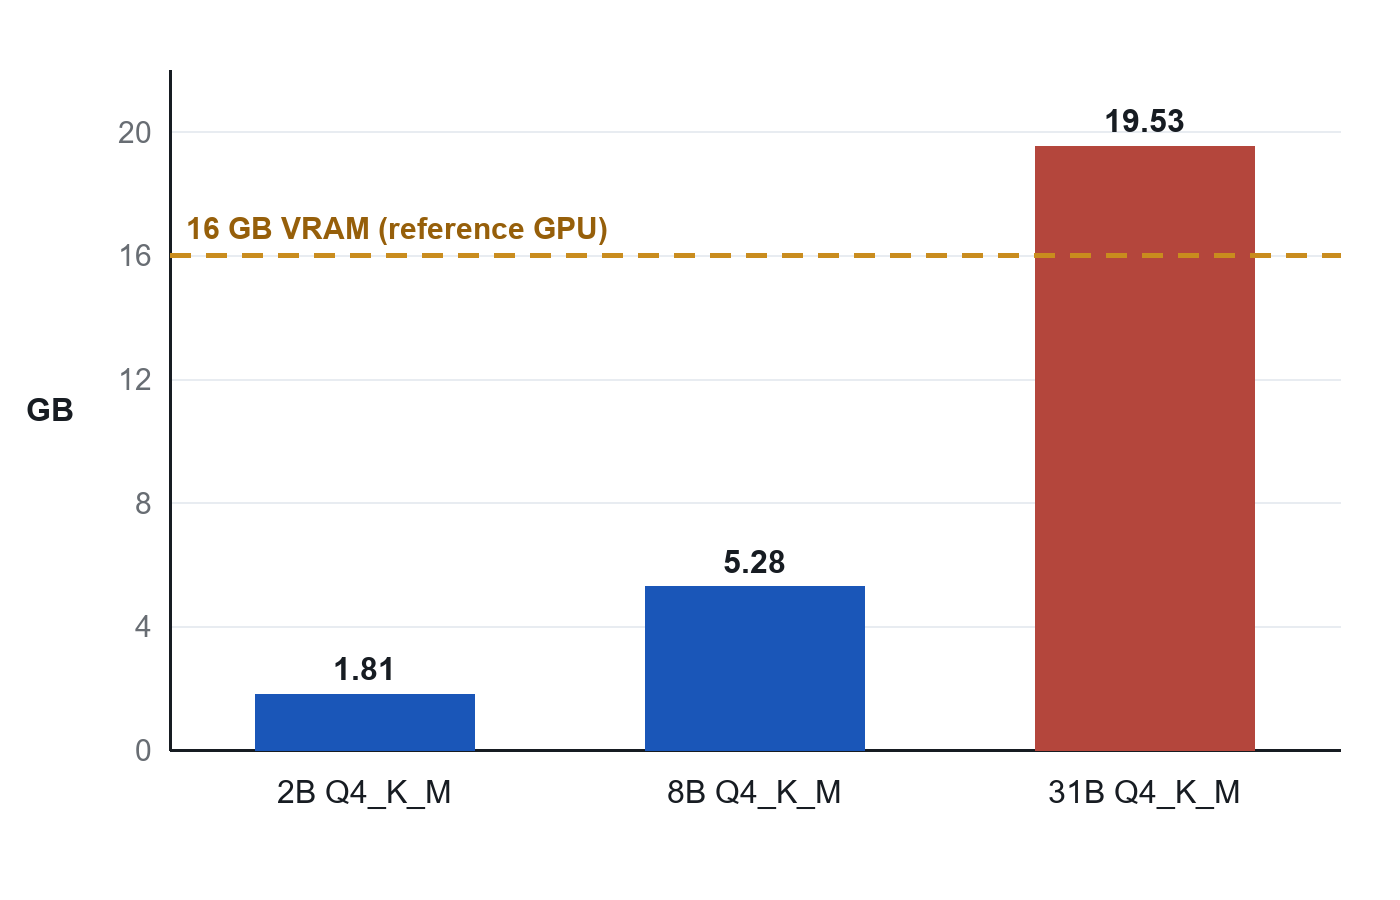
\includegraphics[width=\columnwidth]{fig-model-sizes.png}
  \caption{Model file sizes compared with the 16\,GB video memory of the reference GPU.}
  \label{fig:models}
\end{figure}

\section{Installation}
\label{sec:install}

\subsection{Setup Script}
Double-click \texttt{Start-PLaMoPaperTranslator.cmd}. On the first run it shows the main points of the PLaMo Community License~\cite{plamolicense} and asks for confirmation. The setup script then performs five steps:
\begin{enumerate}
  \item create a Python virtual environment and install pypdf~\cite{pypdf}, Pillow~\cite{pillow} and pypdfium2~\cite{pypdfium2};
  \item download the CUDA build of llama.cpp, or the Vulkan build when no NVIDIA GPU is present;
  \item download the model and its chat template from the official Hugging Face repository;
  \item verify the GGUF header, the file size and the SHA-256 digest;
  \item start the application and open \texttt{http://127.0.0.1:7865}.
\end{enumerate}
Interrupted downloads resume from a \texttt{.partial} file. A model file $f$ is accepted only when
\begin{equation}
  \operatorname{size}(f) = b^\star \quad\wedge\quad \operatorname{SHA256}(f) = h^\star ,
  \label{eq:integrity}
\end{equation}
where $b^\star$ and $h^\star$ are the values currently published by the official repository.

\subsection{Chrome Launcher}
The portable package includes an optional Chrome extension. After loading the extension and running \texttt{install-native-host.ps1}, the toolbar button or \textsc{Alt+Shift+P} restarts the application and opens the reader. If a translation is running, the application is not restarted, so no work is lost.

\section{Document Pipeline}
\label{sec:pipeline}
Figure~\ref{fig:pipeline} summarises how an uploaded file becomes a list of segments. Files of up to 80\,MB in PDF, TXT or Markdown format are accepted.

\begin{figure*}[t]
  \centering
  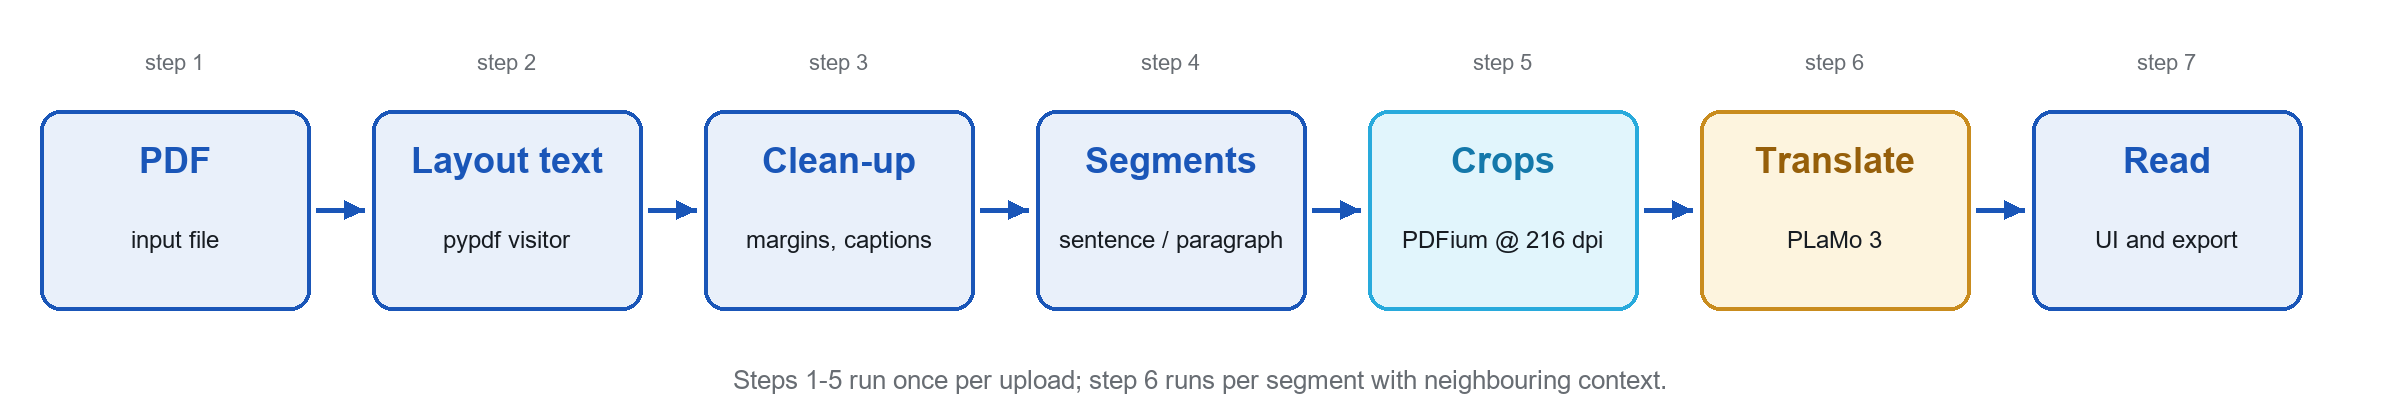
\includegraphics[width=\textwidth]{fig-pipeline.png}
  \caption{Document pipeline. Extraction and clean-up run once per upload; translation runs once per segment.}
  \label{fig:pipeline}
\end{figure*}

\subsection{Text and Layout Extraction}
Text is read with pypdf together with the position and font size of every text fragment. Running headers and footers are removed using these positions. Let $k(\cdot)$ map a small-font fragment near the top or bottom margin to a normalised key. The set of repeated margin keys is
\begin{equation}
  R = \bigl\{\, k \;\big|\; \lvert \{\, p : k \in K_p \,\}\rvert \ge 2 \,\bigr\},
  \label{eq:margins}
\end{equation}
where $K_p$ is the set of keys found on page $p$. Fragments whose key is in $R$ are dropped, as are page numbers.

\subsection{Segmentation}
The cleaned text is split into blocks and each block is classified as a heading, sentence, list item, caption, equation, table or citation. In sentence mode every sentence becomes a segment; in paragraph mode the sentences of one paragraph are kept together. A segment is identified by its paragraph number $p$ and its position $k$ in the paragraph,
\begin{equation}
  s_{p,k}, \qquad p = 1,\dots,P,\quad k = 1,\dots,n_p .
  \label{eq:segment}
\end{equation}
Headings are assigned a level from their numbering, so ``3.2'' becomes level~2. Sentences broken by a page or column boundary are merged again, and each reference entry is merged into a single citation segment.

\subsection{Figures and Equations}
Figures are cropped from the rendered page rather than taken from the embedded images. Labels such as (a) and (b) that are drawn over a figure are therefore kept. A numbered display equation is detected from the position of its number at the right margin and rendered with PDFium at
\begin{equation}
  \sigma = \frac{216\ \text{dpi}}{72\ \text{pt/in}} = 3
  \label{eq:scale}
\end{equation}
pixels per point. The extracted text of the equation is kept for search and copying, but the image is treated as the authoritative form and is never translated.

\section{Translation}
\label{sec:translation}

\subsection{Context Construction}
PLaMo 3 Translate accepts optional context through its chat template~\cite{plamo3}. For segment $s_{p,k}$ the application builds
\begin{equation}
  c_{p,k} = \operatorname{trunc}_{1400}\!\bigl( u \,\Vert\, \operatorname{suf}_{600}(B_{p,k}) \,\Vert\, \operatorname{pre}_{600}(A_{p,k}) \bigr),
  \label{eq:context}
\end{equation}
where $u$ is the reader's own context note, $B_{p,k} = s_{p,1}\cdots s_{p,k-1}$ and $A_{p,k} = s_{p,k+1}\cdots s_{p,n_p}$ are the sentences before and after it in the same paragraph, and $\Vert$ denotes concatenation. Figure~\ref{fig:context} illustrates the construction.

\begin{figure}[t]
  \centering
  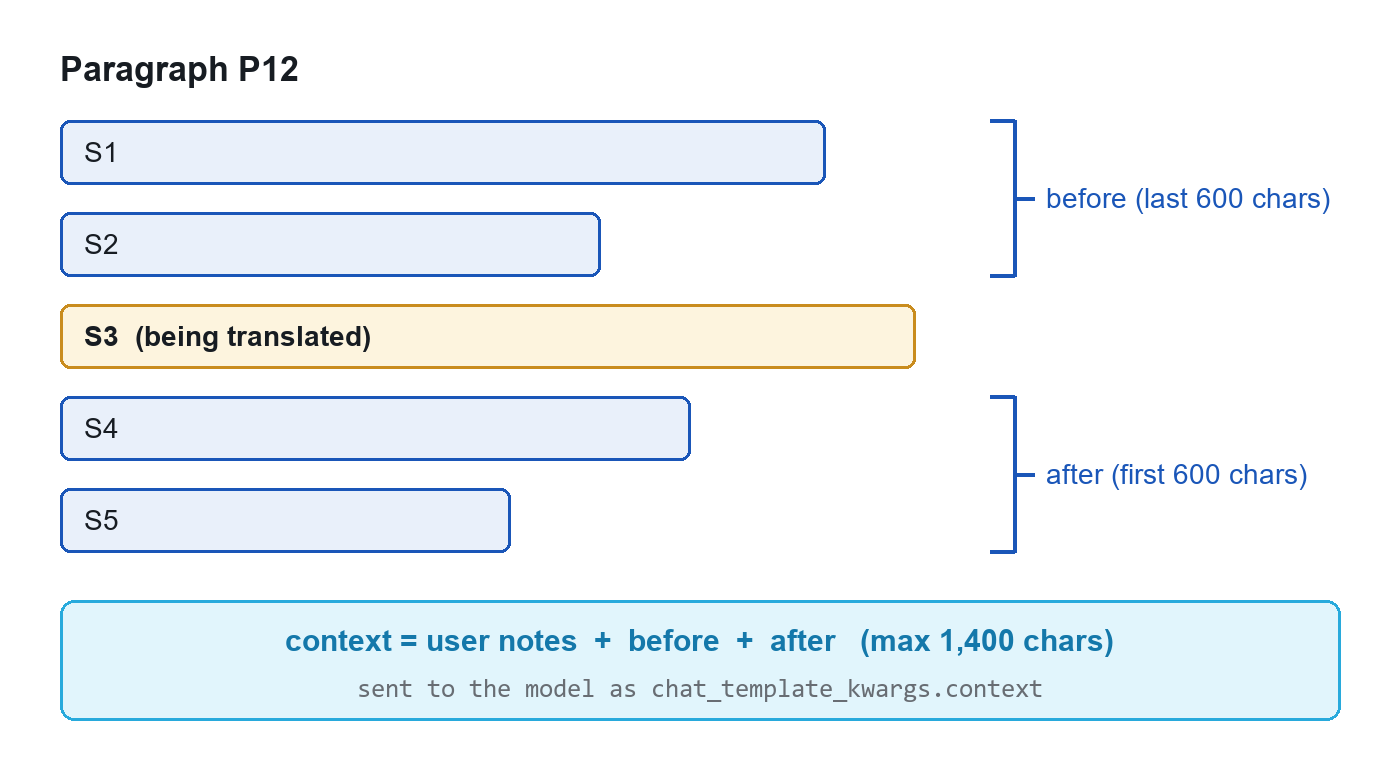
\includegraphics[width=\columnwidth]{fig-context.png}
  \caption{Context for one sentence. Only sentences from the same paragraph are used, so unrelated text never leaks into the prompt.}
  \label{fig:context}
\end{figure}

\subsection{Request Parameters}
Decoding is greedy (temperature $0$). The output limit for a source segment of $n$ characters is
\begin{equation}
  T(n) = \min\bigl(2048,\; \max(384,\; \lfloor 1.35\,n \rfloor)\bigr)
  \label{eq:tokens}
\end{equation}
tokens. Segments that contain almost no letters, such as a row of numbers, are copied unchanged. Algorithm~\ref{alg:translate} shows the complete loop. The job is written to disk every three segments, so at most three translations are lost if the computer stops.

\begin{algorithm}[t]
  \caption{Translation job}
  \label{alg:translate}
  \begin{algorithmic}[1]
    \Require segments $s_1,\dots,s_N$, options $\theta$
    \State start llama-server if it is not healthy
    \For{$i = 1$ \textbf{to} $N$}
      \If{the job was cancelled} \State \Return cancelled \EndIf
      \If{$s_i$ is an equation with an image}
        \State $t_i \gets s_i$
      \Else
        \State $t_i \gets \textsc{Translate}(s_i, c_i, \theta)$
      \EndIf
      \If{$i \bmod 3 = 1$} \State save job \EndIf
    \EndFor
    \State \Return completed
  \end{algorithmic}
\end{algorithm}

\subsection{Glossary}
A glossary fixes the translation of important terms. Each line holds one source term and its required translation; the accepted separators are listed in Table~\ref{tab:glossary}. Lines starting with \texttt{\#} are comments. In the table, \textit{T} stands for the term in the target language.

\begin{table}[t]
  \centering
  \caption{Glossary syntax. All four lines define the same pair.}
  \label{tab:glossary}
  \begin{tabular}{@{}ll@{}}
    \toprule
    Line & Separator \\
    \midrule
    \texttt{curved layer = }\textit{T} & equals sign \\
    \texttt{curved layer => }\textit{T} & ASCII arrow \\
    \texttt{curved layer }\textrightarrow{}\ \textit{T} & Unicode arrow \\
    \texttt{curved layer<TAB>}\textit{T} & tab character \\
    \bottomrule
  \end{tabular}
\end{table}

\subsection{Progress}
While a job runs, the progress shown to the reader after $m$ of $N$ segments is
\begin{equation}
  \pi = \frac{1}{10}\operatorname{round}\!\left( 1000 \cdot \frac{m}{N} \right) \%,
  \label{eq:progress}
\end{equation}
that is, a percentage rounded to one decimal place.

\section{Reading Interface}
\label{sec:reader}

\subsection{Layout}
The reader is not tied to the page size of the PDF. On a wide screen the outline is fixed on the left and the bookmark list on the right, as in Figure~\ref{fig:reader}. On a tablet both lists move above the text, and on a narrow screen the note field moves below each pair.

\subsection{Navigation and Cross-References}
References such as ``Fig.~3'', ``Eq.~(2)'' and ``Table~1'' become links. When several segments carry the same number, the one with an image is preferred. Each jump is recorded, and the \emph{Back} button returns to the previous position; the last 20 positions are kept. A figure that appears in the PDF far from its first mention is moved to just after that mention.

\subsection{Notes, Bookmarks and Clips}
Each segment has a note field that is saved automatically, and a star that adds it to the bookmark list. The source, translation or note of any segment can be \emph{clipped}; clips stay visible in the lower-right corner while reading. If $C_i \subseteq \{\text{source}, \text{translation}, \text{note}\}$ denotes the parts clipped from segment $i$, the application enforces
\begin{equation}
  \sum_{i=1}^{N} \lvert C_i \rvert \le 3 .
  \label{eq:clips}
\end{equation}
Figure~\ref{fig:panels} shows the outline and the clip shelf.

\begin{figure}[t]
  \centering
  \begin{subfigure}[b]{0.47\columnwidth}
    \centering
    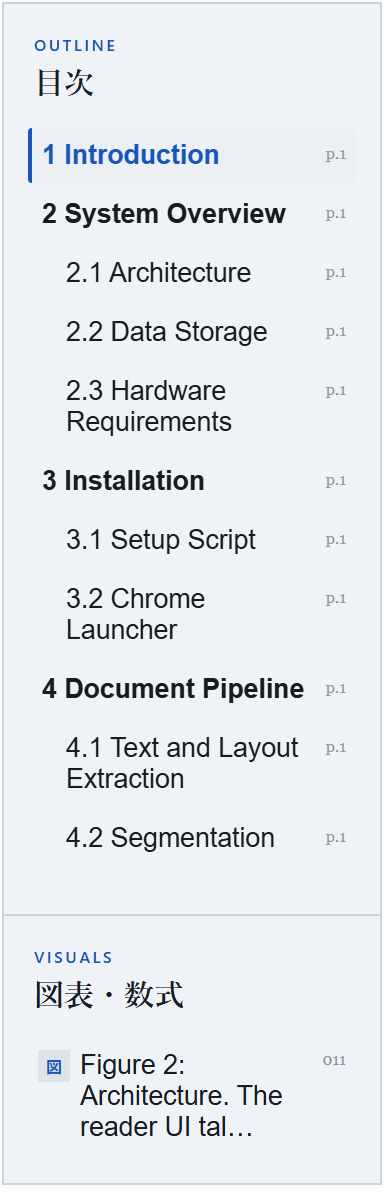
\includegraphics[width=\textwidth]{fig-outline.png}
    \caption{Outline}
    \label{fig:panels-outline}
  \end{subfigure}\hfill
  \begin{subfigure}[b]{0.47\columnwidth}
    \centering
    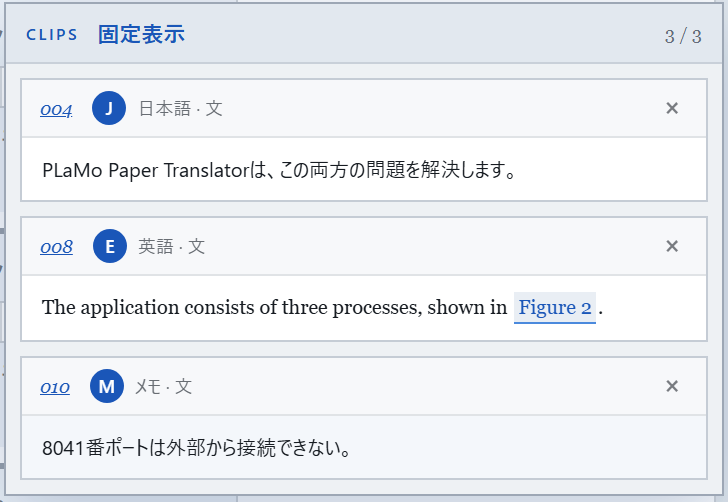
\includegraphics[width=\textwidth]{fig-clips.png}
    \caption{Clip shelf}
    \label{fig:panels-clips}
  \end{subfigure}
  \caption{Reading aids: (a) the outline generated from headings and (b) the clip shelf with pinned segments.}
  \label{fig:panels}
\end{figure}

\subsection{Editing and Retranslation}
The \emph{Edit} button corrects a single translation. \emph{Retranslate} sends one segment to the model again with the same context and glossary. The previous text is kept as a revision; up to 20 revisions per segment can be viewed and restored. Equation images cannot be edited.

\subsection{Keyboard Shortcuts}
Table~\ref{tab:shortcuts} lists the shortcuts.

\begin{table}[t]
  \centering
  \caption{Keyboard shortcuts.}
  \label{tab:shortcuts}
  \begin{tabular}{@{}ll@{}}
    \toprule
    Keys & Action \\
    \midrule
    \textsc{Alt+L} & open the library \\
    \textsc{Alt+S} & open the paper summary \\
    \textsc{Alt+Shift+P} & restart and open (Chrome) \\
    \textsc{Esc} & close the current dialog \\
    \bottomrule
  \end{tabular}
\end{table}

\section{Quality Check}
\label{sec:quality}
The quality check finds problems that can be detected mechanically. It does not replace proofreading by a person. Table~\ref{tab:quality} lists the checks. For a source $s$ and translation $t$, a translation is reported as suspiciously short when
\begin{equation}
  \lvert s \rvert \ge 80 \quad\wedge\quad \lvert t \rvert < \max\bigl(8,\; \lfloor 0.12\,\lvert s \rvert \rfloor\bigr),
  \label{eq:short}
\end{equation}
and numbers are reported when the set difference
\begin{equation}
  M = \mathcal{N}(s) \setminus \mathcal{N}(t)
  \label{eq:numbers}
\end{equation}
is not empty, where $\mathcal{N}(\cdot)$ extracts numbers together with \%, \textdegree C and \textdegree F.

\begin{table}[t]
  \centering
  \caption{Checks performed by the quality check.}
  \label{tab:quality}
  \begin{tabular}{@{}lll@{}}
    \toprule
    Check & Level & Condition \\
    \midrule
    Missing & error & no translation \\
    Unchanged & warning & $t = s$, $\ge 3$ words \\
    Numbers & warning & Eq.~(\ref{eq:numbers}) \\
    Short & warning & Eq.~(\ref{eq:short}) \\
    Glossary & info & target term absent \\
    \bottomrule
  \end{tabular}
\end{table}

\section{Paper Library}
\label{sec:library}
The library lists every saved translation (Figure~\ref{fig:library}). It searches titles, tags, summaries, source text, translations and notes, and filters by reading status: unread, reading, completed or archived. Opening a paper resumes at the last segment read. For a paper with $N$ segments whose last read segment has index $r$ (counting from zero), the progress bar shows
\begin{equation}
  \rho = \operatorname{round}\!\left( 100 \cdot \frac{r + 1}{N} \right) \%.
  \label{eq:reading}
\end{equation}

\begin{figure}[t]
  \centering
  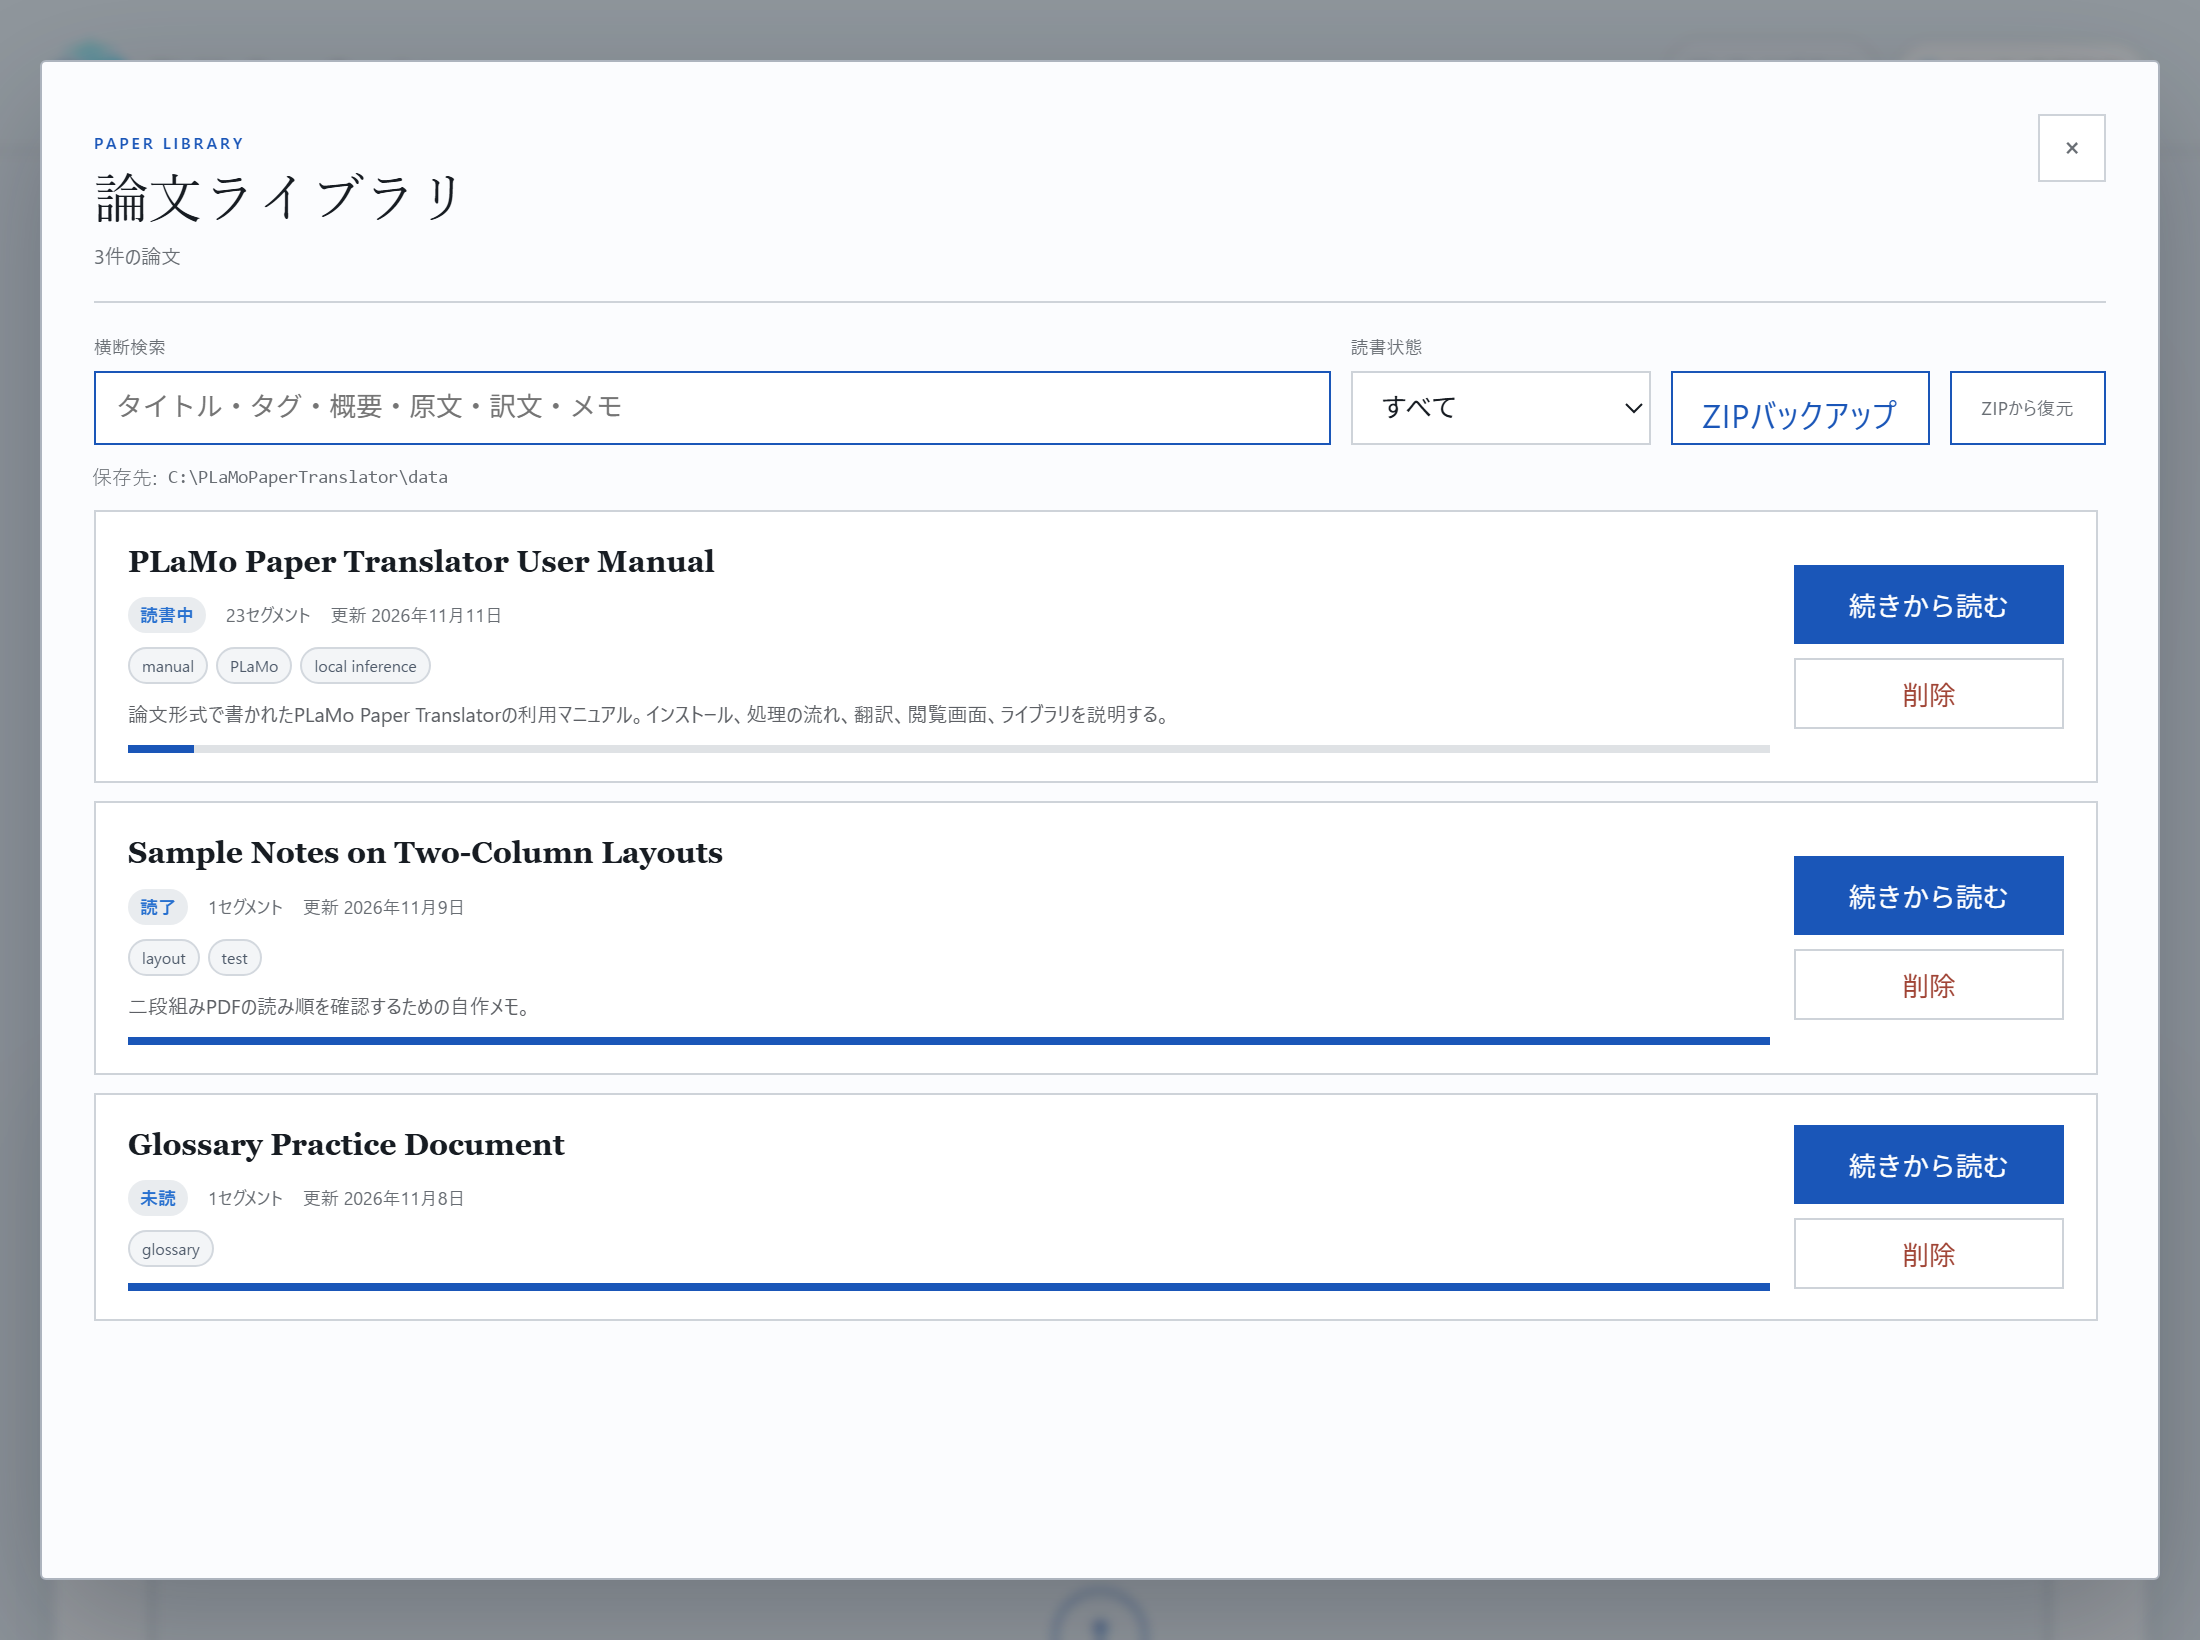
\includegraphics[width=\columnwidth]{fig-library.png}
  \caption{The paper library with search, reading-status filter, backup and restore.}
  \label{fig:library}
\end{figure}

\subsection{Backup and Restore}
\emph{ZIP backup} saves jobs, original files and crops in one archive. \emph{Restore from ZIP} only adds files that do not exist yet; it never overwrites. Before anything is written, the archive must satisfy
\begin{align}
  \text{upload size} &\le 2\ \text{GB}, \label{eq:backup-upload}\\
  \textstyle\sum \text{expanded size} &\le 8\ \text{GB}, \label{eq:backup-expanded}\\
  \text{number of files} &\le 100{,}000, \label{eq:backup-files}
\end{align}
and every path must lie inside \texttt{data/jobs}, \texttt{data/uploads} or \texttt{data/assets}.

\subsection{Deleting a Paper}
\emph{Delete} removes a translation after confirmation. The original file and crops are deleted as well, unless another translation was made from the same file. A paper that is being translated cannot be deleted.

\section{Export and Licensing}
\label{sec:export}
Table~\ref{tab:export} lists the export formats. Every export carries the attribution ``Built with PLaMo'' and names the model, as required by the PLaMo Community License~\cite{plamolicense}. Use within an organisation can count as commercial use under that license; check its conditions before deploying the application at work.

\begin{table}[t]
  \centering
  \caption{Export formats.}
  \label{tab:export}
  \begin{tabular}{@{}lp{0.62\columnwidth}@{}}
    \toprule
    Format & Contents \\
    \midrule
    HTML & single file with embedded figures and notes \\
    Markdown & source and translation, one pair per entry \\
    JSON & all segments, tags, summary and reading status \\
    \bottomrule
  \end{tabular}
\end{table}

When publishing translations of other people's papers, check the license of each paper. A license that allows adaptation, such as CC BY 4.0~\cite{ccby}, is required, because a translation is an adapted work.

\section{Limitations}
\label{sec:limitations}
The application needs a PDF that contains text; scanned pages must be processed with OCR first. Two-column layouts are read in the order stored in the PDF, which is usually but not always the reading order. Figures drawn only with vector graphics are not cropped, and their text is kept as ordinary segments. Inline mathematics is translated as text. Finally, machine translation can be wrong: results used for submissions, contracts or medical decisions must be checked by an expert.

\section{Conclusion}
\label{sec:conclusion}
PLaMo Paper Translator brings structure-aware, sentence-level translation of academic papers to an ordinary laptop without sending any text to the cloud. We hope this manual is useful both as a guide and as a test document. Because it is dedicated to the public domain, it can be translated, shown in videos and redistributed without restriction.

\section*{Acknowledgments}
The application is built with PLaMo. It relies on llama.cpp, pypdf, Pillow and PDFium, and we thank their developers.

\begin{thebibliography}{9}
\bibitem{plamo3}
Preferred Networks, Inc.
\newblock PLaMo 3 Translate 8B (GGUF).
\newblock \url{https://huggingface.co/pfnet/plamo-3-translate-8b-GGUF}, 2026.

\bibitem{plamolicense}
Preferred Networks, Inc.
\newblock PLaMo Community License.
\newblock \url{https://plamo.preferredai.jp/info/plamo-community-license-ja}.

\bibitem{llamacpp}
G.~Gerganov and contributors.
\newblock llama.cpp: LLM inference in C/C++.
\newblock \url{https://github.com/ggml-org/llama.cpp}.

\bibitem{pypdf}
pypdf contributors.
\newblock pypdf: a pure-Python PDF library.
\newblock \url{https://pypdf.readthedocs.io/}.

\bibitem{pypdfium2}
pypdfium2 contributors.
\newblock pypdfium2: Python bindings to PDFium.
\newblock \url{https://github.com/pypdfium2-team/pypdfium2}.

\bibitem{pillow}
J.~A.~Clark and contributors.
\newblock Pillow: the friendly PIL fork.
\newblock \url{https://python-pillow.org/}.

\bibitem{nativemessaging}
Google.
\newblock Native messaging.
\newblock Chrome for Developers documentation, \url{https://developer.chrome.com/docs/extensions/develop/concepts/native-messaging}.

\bibitem{ccby}
Creative Commons.
\newblock Attribution 4.0 International (CC BY 4.0).
\newblock \url{https://creativecommons.org/licenses/by/4.0/}.

\bibitem{cc0}
Creative Commons.
\newblock CC0 1.0 Universal Public Domain Dedication.
\newblock \url{https://creativecommons.org/publicdomain/zero/1.0/}.
\end{thebibliography}

\appendix
\section{HTTP Interface}
\label{app:api}
Table~\ref{tab:api} lists the main endpoints of \texttt{app.py}. They are intended for the bundled reader and the Chrome launcher~\cite{nativemessaging}; they are not a stable public interface.

\begin{table}[h]
  \centering
  \caption{Main HTTP endpoints.}
  \label{tab:api}
  \small
  \begin{tabular}{@{}ll@{}}
    \toprule
    Request & Purpose \\
    \midrule
    \texttt{GET /api/status} & engine and model state \\
    \texttt{POST /api/documents} & upload and extract a file \\
    \texttt{POST /api/jobs} & start a translation \\
    \texttt{GET /api/jobs/\{id\}} & job state and segments \\
    \texttt{GET /api/jobs/\{id\}/export} & HTML, MD or JSON \\
    \texttt{GET /api/jobs/\{id\}/quality} & quality check \\
    \texttt{DELETE /api/jobs/\{id\}} & delete a paper \\
    \texttt{GET /api/library} & search the library \\
    \bottomrule
  \end{tabular}
\end{table}

\section{Troubleshooting}
\label{app:trouble}
\begin{itemize}
  \item \textbf{The engine does not start.} Check \texttt{data/llama-server.log}. Loading must finish within three minutes.
  \item \textbf{Nothing is extracted.} The PDF probably contains only images; run OCR first.
  \item \textbf{The Chrome button reports an error.} Run \texttt{install-native-host.ps1} again and restart Chrome.
\end{itemize}

\vspace{6pt}
\noindent\small This manual is dedicated to the public domain under CC0 1.0~\cite{cc0}. It may be copied, translated and redistributed for any purpose without permission or attribution.

\end{document}
